%% BioMed_Central_Tex_Template_v1.06

%%% additional documentclass options:
%  [doublespacing]
%  [linenumbers]   - put the line numbers on margins

%%% loading packages, author definitions

%\documentclass[twocolumn]{bmcart}% uncomment this for twocolumn layout and comment line below
\documentclass[doublespacing]{configs/bmcart}

%%% Load packages
%\usepackage{amsthm,amsmath}
%\RequirePackage{natbib}
%\RequirePackage[authoryear]{natbib}% uncomment this for author-year bibliography
%\RequirePackage{hyperref}
%\usepackage[utf8]{inputenc} %unicode support
%\usepackage[applemac]{inputenc} %applemac support if unicode package fails
%\usepackage[latin1]{inputenc} %UNIX support if unicode package fails
\usepackage{booktabs}
\usepackage{graphicx}
\usepackage{hyperref}
\hypersetup{
    colorlinks=false,
    linkcolor=black,
    filecolor=black,      
    urlcolor=black,
}
\usepackage{url}
\usepackage{amsmath} % small matrix package
\usepackage[left]{lineno} % linenumbers
\linenumbers

\usepackage[acronym]{glossaries}

%\makenoidxglossaries
\makeglossaries
\newacronym{roi}{ROI}{region of interest}
\newacronym{sfm}{SfM-MVS}{structure-from-motion multi-view stereo photogrammetry}
\newacronym{dom}{DOM}{digital orthophoto map}
\newacronym{dsm}{DSM}{digital surface model}
\newacronym{pcd}{PCD}{point cloud data}
\newacronym{gis}{GIS}{geographic information system}
\newacronym{gcp}{GCPs}{ground control points}
\newacronym{mtp}{MTPs}{manual tie points}
\newacronym{mkl}{MKL}{math kernel library}
\newacronym{gui}{GUI}{graphical user interface}
\newacronym{iou}{IoU}{intersection of union}
\newacronym{rtk}{RTK}{real-time kinematic}
\newacronym{pmvs}{PMVS}{patch-based multi-view stereo}
\newacronym{pcl}{PCL}{point cloud library}


%%%%%%%%%%%%%%%%%%%%%%%%%%%%%%%%%%%%%%%%%%%%%%%%%
%%                                             %%
%%  If you wish to display your graphics for   %%
%%  your own use using includegraphic or       %%
%%  includegraphics, then comment out the      %%
%%  following two lines of code.               %%
%%  NB: These line *must* be included when     %%
%%  submitting to BMC.                         %%
%%  All figure files must be submitted as      %%
%%  separate graphics through the BMC          %%
%%  submission process, not included in the    %%
%%  submitted article.                         %%
%%                                             %%
%%%%%%%%%%%%%%%%%%%%%%%%%%%%%%%%%%%%%%%%%%%%%%%%%

%\def\includegraphic{}
%\def\includegraphics{}


%%% Put your definitions there:
%\startlocaldefs
%\endlocaldefs


%%% Begin ...
\begin{document}

%%% Start of article front matter
\begin{frontmatter}

\begin{fmbox}
\dochead{Software}

%%%%%%%%%%%%%%%%%%%%%%%%%%%%%%%%%%%%%%%%%%%%%%
%%                                          %%
%% Enter the title of your article here     %%
%%                                          %%
%%%%%%%%%%%%%%%%%%%%%%%%%%%%%%%%%%%%%%%%%%%%%%

\title{EasyRIC: A python package for annotation transformation among photogrammetry 3D reconstruction products}

%%%%%%%%%%%%%%%%%%%%%%%%%%%%%%%%%%%%%%%%%%%%%%
%%                                          %%
%% Enter the authors here                   %%
%%                                          %%
%% Specify information, if available,       %%
%% in the form:                             %%
%%   <key>={<id1>,<id2>}                    %%
%%   <key>=                                 %%
%% Comment or delete the keys which are     %%
%% not used. Repeat \author command as much %%
%% as required.                             %%
%%                                          %%
%%%%%%%%%%%%%%%%%%%%%%%%%%%%%%%%%%%%%%%%%%%%%%

\author[
   addressref={aff1},
   %email={haozhou-wang@g.ecc.u-tokyo.ac.jp}
]{\inits{HW}\fnm{Haozhou} \snm{Wang}}
\author[
   addressref={aff1},
   corref={aff1}, 
   email={guowei@g.ecc.u-tokyo.ac.jp}
]{\inits{WG}\fnm{Wei} \snm{Guo}}

%%%%%%%%%%%%%%%%%%%%%%%%%%%%%%%%%%%%%%%%%%%%%%
%%                                          %%
%% Enter the authors' addresses here        %%
%%                                          %%
%% Repeat \address commands as much as      %%
%% required.                                %%
%%                                          %%
%%%%%%%%%%%%%%%%%%%%%%%%%%%%%%%%%%%%%%%%%%%%%%

\address[id=aff1]{
  \orgname{International Field Phenomics Research Laboratory, Institute for Sustainable Agro-ecosystem Services, Graduate School of Agricultural and Life Science, The University of Tokyo}, 
  \postcode{188-0002} 
  \city{Tokyo}, 
  \cny{Japan}
}

%%%%%%%%%%%%%%%%%%%%%%%%%%%%%%%%%%%%%%%%%%%%%%
%%                                          %%
%% Enter short notes here                   %%
%%                                          %%
%% Short notes will be after addresses      %%
%% on first page.                           %%
%%                                          %%
%%%%%%%%%%%%%%%%%%%%%%%%%%%%%%%%%%%%%%%%%%%%%%

%\begin{artnotes}
%%\note{Sample of title note}     % note to the article
%\note[id=n1]{Equal contributor} % note, connected to %author
%\end{artnotes}

\end{fmbox}% comment this for two column layout

%%%%%%%%%%%%%%%%%%%%%%%%%%%%%%%%%%%%%%%%%%%%%%
%%                                          %%
%% The Abstract begins here                 %%
%%                                          %%
%% Please refer to the Instructions for     %%
%% authors on http://www.biomedcentral.com  %%
%% and include the section headings         %%
%% accordingly for your article type.       %%
%%                                          %%
%%%%%%%%%%%%%%%%%%%%%%%%%%%%%%%%%%%%%%%%%%%%%%

\begin{abstractbox}

\begin{abstract}
\parttitle{Background} 
Applying 3D based high-throughput phenotyping in agriculture provides an advanced and efficient method for managing and monitoring crops. The \acrfull*{sfm}, applicable to common RGB digital cameras, has been widely used to implement this task by many commercial and open-source tools. However, analyzing its outputs, including \acrfull*{dom}, \acrfull*{dsm}, and \acrfull*{pcd}, for high-throughput plant phenotyping, requires several preprocessing steps, such as \acrfull*{roi} extraction,  plot segmentation, or object detection. Currently, there is no easy-to-use tool to meet this requirement.

\parttitle{Results}
In this study, a pure python package called EasyRIC (easy reconstruction image converter) was developed to link the outputs of \acrshort*{sfm} products with original photos. The Lotus (\textit{Nelumbo nucifera}) breeding field were used to demonstrate the following points: 1) clipping (segmenting) \acrshort*{sfm} products according to given plot boundary or \acrshort*{roi}. 2) transforming ROI on the \acrshort*{sfm} products to high quality raw images to assist object detection. 3) evaluating the accuracy of previous transformation by manual annotation.

\parttitle{Conclusions}
This method shows an acceptable accuracy and potential to preprocess those outputs of \acrshort*{sfm}. The suggestions for better reverse calculation have been discussed. Also, some potential applications for deep learning have also been proposed.

\end{abstract}

%%%%%%%%%%%%%%%%%%%%%%%%%%%%%%%%%%%%%%%%%%%%%%
%%                                          %%
%% The keywords begin here                  %%
%%                                          %%
%% Put each keyword in separate \kwd{}.     %%
%%                                          %%
%%%%%%%%%%%%%%%%%%%%%%%%%%%%%%%%%%%%%%%%%%%%%%

\begin{keyword}
\kwd{Orthomosaic}
\kwd{photogrammetry}
\kwd{Phenotyping}
\kwd{Reverse calculation}
\end{keyword}

\end{abstractbox}
%
%\end{fmbox}% uncomment this for twocolumn layout

\end{frontmatter}

%%%%%%%%%%%%%%%%%%%%%%%%%%%%%%%%%%%%%%%%%%%%%%
%%                                          %%
%% The Main Body begins here                %%
%%                                          %%
%% Please refer to the instructions for     %%
%% authors on:                              %%
%% http://www.biomedcentral.com/info/authors%%
%% and include the section headings         %%
%% accordingly for your article type.       %%
%%                                          %%
%% See the Results and Discussion section   %%
%% for details on how to create sub-sections%%
%%                                          %%
%% use \cite{...} to cite references        %%
%%  \cite{koon} and                         %%
%%  \cite{oreg,khar,zvai,xjon,schn,pond}    %%
%%  \nocite{smith,marg,hunn,advi,koha,mouse}%%
%%                                          %%
%%%%%%%%%%%%%%%%%%%%%%%%%%%%%%%%%%%%%%%%%%%%%%

\section*{Background}
Compared with traditional manual field mensuration which is time-consuming, labor intensive, and subjectivity inevitable, the recent developed 3D reconstruction technique provides a high-throughput solution for structural trait estimation. The \acrfull*{sfm} 3D reconstruction technology, independent of specific instructions except common digital camera, has been widely used in plant phenotyping study area \cite{jay_field_2015, sun_three-dimensional_2020, zhu_quantification_2020}, by analyzing it produced \acrfull*{pcd} or geographic products like \acrfull*{dom} and \acrfull*{dsm}.

% how the outputs been used differently indoor and outdoor
Current application of SfM-MVS in phenotyping area could be split to indoor and outdoor. For indoor application, the DOM and DSM are not the mandatory outputs. Many indoor studies proved the feasibility of \acrshort*{sfm} technology to build PCD of individual crops with good quality \cite{wang_maize_2019, rossi_performances_2020}, and the visually close to that obtained by LiDAR \cite{thapa_novel_2018} and RGB-Depth camera \cite{martinez-guanter_low-cost_2019}. Several studies focused on developing algorithms to classify or segment point clouds, and then calculate geometry traits from previous results \cite{ziamtsov_machine_2019, artzet_phenomenal_2019}. While for outdoor experimental fields application, though PCD is also an important data source for crop modeling and traits extraction \cite{jay_field_2015, sun_three-dimensional_2020, zhu_quantification_2020}, the DOM and DSM are also required for plot management and simplify the crop analyzing difficulties \cite{sun_field_2018, tresch_easympe_2019, chen_grid_2020}. Aligning the SfM outputs of different time also showed the ability for time-series analysis \cite{dong_4d_2017, han_clustering_2018}.

% The current challenges that using DOM PCD and DSM
Though the feasibility of applying SfM products into plant phenotyping has been validated by many studies, there are still several pain points exist in preprocessing stage. For one thing, the size of SfM outputs (DOM, DSM, PCD) is not so convenient to use. The DOM and PCD in the field often have unused background, gathering them into one file making data analyzing and plot tracking more complicated. Hence, one common preprocessing is clipping those outputs according to plot sectors or \acrfull*{roi}, and making it easier for plot management and benefit for time-series analysis. For another, effected by light condition and plant leaf movement by wind, it is difficult to avoid the "ghost effect" on produced DOM and also hard to obtain the same quality as raw images for image-based trait calculation. Hence, finding the correspondent position from ROI on DOM or PCD to high quality raw images would contribute to the accuracy improvement by image analysis.

The objective of this study, is developing an easy-to-use software package to solve previous pain points in SfM-MVS outputs preprocessing for plant phenotyping, including: 1) clipping produced DOM or PCD data to small parts or sectors, follows the given plot boundary or ROI. 2) connecting and transforming the ROI from SfM-MVS outputs to high quality raw images. 3) testing the accuracy and performance of previous transformation by a case study.

\section*{Implementation}

An open-source python package called EasyRIC (easy reconstruction image converter) was implemented to manipulating \acrshort*{sfm} software outputs and raw images. Though the source codes were cross-platform due to the characteristic of python language, they were programmed and tested under Windows 10 64-bit platform and Intel CPU with \acrfull*{mkl}. For achieve better package performance, the 8 GB RAM and 3.0 GHz CPU are recommended. The source code and user manual can be accessed via: \url{https://github.com/HowcanoeWang/EasyRIC}, the License is GPL-3.0 which is free to use for any purpose.

The general workflow of this tool was shown in Figure \ref{fig:workflow}. There were three main parts of this workflow, including two input data preparations: a) 3D reconstruction outputs and b) making \acrshort*{roi} by other tools; and c) EasyRIC functions, highly correspondence with 3D reconstruction workflow: (1) SfM stage, (2) MVS stage, and (3) \acrfull*{gis} stage respectively. 

\subsection*{Input data preparation}

\subsubsection*{Image collection and 3D reconstruction}
% image collection
The quality of raw image is the fundamental of \acrshort*{sfm} process as well as the EasyRIC package. The images with balanced brightness, exposure, and minimum motion blur are of great importance. Over 50\% overlapping among each adjacent images is also recommended. Though \acrfull*{gcp} or \acrfull*{mtp}, or even \acrfull*{rtk} are optional for \acrshort*{sfm} software. It is strongly recommended to set several object or tags or scale bars to calibrate and define geographic positions. One option is Chilitags (\url{https://github.com/chili-epfl/chilitags}), the automatic workflow decrease a plenty of workloads in current \acrshort*{sfm} software.

% SfM workflow
After getting acceptable quality image data, the \acrshort*{sfm} workflow is required. Currently, there are several \acrshort*{sfm} software available, can be split into commercial and open-source ones. The common used commercial software includes Pix4Dmapper and Agisoft Metashape and for open-source software, OpenMVG \cite{openmvg_openmvg_2020}, libMV \cite{mierle_libmv_2020}, VisualSFM \cite{wu_visualsfm_2020}, Bundler \cite{snavely_bundler_2020}, and FieldReconst \cite{naro_fieldreconst_2020} are included. Compared with commercial software, most of the open-source software can not deal with the full process of \acrshort*{sfm}, as Zhu et al., \cite{zhu_quantification_2020} and Hui et al., \cite{hui_image-based_2018} applied in their projects, VisualSFM, \acrfull*{pmvs} \cite{furukawa_accurate_2010}, \acrfull*{pcl} \cite{rusu_3d_2011}, and Geomagic Studio software (Raindrop Geomagic, Morrisville, NC, USA) are used to implement the full process which embedded in Pix4Dmapper. For this study, the commercial Pix4Dmapper was used as its default setting to produce required camera parameters (pmatrix, external and internal parameters), \acrshort*{pcd}, and GIS products \acrshort*{dom} and \acrshort*{dsm}, and all outputs of Pix4DMapper have been supported and tested. For the future, other commercial software or open source software will be supported.

\subsubsection*{Region of Interest (ROI) making}
Currently, the EasyRIC package has no \acrfull*{gui} for manual \acrshort*{roi} marking. So different external software to marking ROI on different stage outputs are required.

For the SfM stage, which requires obtaining 2D pixel coordinates on raw images, common photo processing software can be used, e.g. open-source GIMP or commercial Photoshop, these software programs display the pixel coordinate where mouse hover. Then these 2D coordinate can be copied or write to txt file or csv file for EasyRIC importing. Also, other deep learning annotation software which produce json annotation files also supported and recommended, for example, LabelMe (\url{https://github.com/wkentaro/labelme}) has been tested and supported in this package.

For the MVS stage, which produces 3D \acrshort*{pcd}, the 3D coordinate is required. Common point cloud processing software which can pick point cloud points and get the 3D coordinate of each point could be used (e.g. CloudCompare, MeshLab, etc.). The open-source CloudCompare (\url{http://cloudcompare.org/}) has been tested in this project and support export picked points coordinates to txt file for later usage. The tutorial for using CloudCompare to make ROI can be referred on our package documentation. For the future, importing the AutoCAD 3D polygon file (*.dxf) will be supported.

For the GIS stage, which requires obtaining 2D geographic coordinates on DOM and DSM, common GIS processing software including QGIS (open source) or ArcMap (commercial) can be used to produce required polygon shapefiles (*.shp). The produced shp file can be used as the input for EasyRIC package.

\subsection*{Package Algorithms}
This section demonstrates how the calculation algorithm implemented, for the specific usage documentation, please refer \url{https://github.com/HowcanoeWang/EasyRIC/wiki}.

\subsubsection*{Input and output files}
% supported file types
The input file type required for this package includes: pix4d camera parameters, pix4d joint rotation-translation matrix (pmatrix) file (*.txt), digital images (*jpeg, *png), point cloud data (*.pcd, *.ply, *.xyz), geotiff files (*.tiff, DOM and DSM), polygon shapefile (*.shp), shapefile geographic projection file (*.prj), and in the future, 3D polygon file (*.dxf).

% packages used
Several external python site-packages were used to deal with these files, all these data were stored as \textit{numpy.ndarray} based data structure for faster matrix algebra calculation. The *.txt pure text files can be read into \textit{ndarray} by \textit{numpy} package, as stored an index python class linked to each raw image name. For *.jpeg and *.png files, the \textit{scikit-image.io.imread} module was used to load image into \textit{numpy.ndarray} format. For point cloud files, the \textit{open3d.io.read\_pcd} module was used, and for Pix4Dmapper produced *.ply files, sometimes the color information can not be correctly loaded, the \textit{plyfile} package was used to compensate the color loss. For the geotiff file, the \textit{tifffile} package was used to load both image layer data to \textit{numpy.ndarray} and geo-header data which contain the offset, resolution, and geographic projection information, helpful for the transformation between pixel coordinate and geographic coordinate on geotiff images. The *.prj file can be read directly by python but \textit{pyproj} package is used to convert pure text to python geo-projection class, and functioned as a projection converter once the shp projection was not the same with geotiff projection. For 3D polygon *.dxf file, the \textit{ezdxf} package was used to convert to \textit{numpy.ndarray} polygon.

% clip & output files
By importing all these materials into the EasyRIC package, a clip function is provided to clip both point cloud data and geotiff GIS map into small sectors by given ROI polygon coordinates. Then these sectors could be saved as the same file type into disk.

\subsubsection*{Geometry from real world to image pixel}
In the geometry between image and real world, there are three coordinates, the first one is the real world geographic coordinate ($xyz_{geo}$, unit is m), the second one is the offset camera coordinate ($xyz_{cam}$), which makes camera position to the origin (0,0,0) of coordinates and the camera medial axis is used as z axis, the last one is the raw image pixel coordinate ($xy_{pix}$, unit is pixel). 

As shown in Figure \ref{fig:geom}.a, assume a point $K(X,Y,Z)$ in real world coordinate ($xyz_{geo}$) is recorded as $k_2$ in image $raw_2$ by camera. For internal parameters, $w$ and $l$ represents the camera sensor width (horizontal) and length (vertical) in mm, respectively, and $f$ is camera focal length in mm. For external camera parameters, the camera rotation and position are recorded by $r_i (\omega_i, \varphi_i, \kappa_i)$ \cite{pix4d_support_yaw_2020} and $P_i (Px_{i}, Py_{i}, Pz_{i})$. The rotation matrix ($\mathbf{R}_i$) of camera parameters 
can be calculated by \cite{pix4d_support_how_2020}, or for Pix4D, can be loaded from \textit{calibrated\_camera\_parameters.txt} file:

$$
\begin{array}{lll}
  \mathbf{R}_i & = & \mathbf{R}_{x_i}(\omega_i) \mathbf{R}_{y_i}(\varphi_i) \mathbf{R}_{z_i}(\kappa_i) \nonumber \\
  & = &
    \begin{small}
    \left[ 
      % amsmath package is required
      \begin{matrix} 
        1 & 0             & 0 \\
        0 & cos(\omega_i) & -sin(\omega_i) \\
        0 & sin(\omega_i) & cos(\omega_i)
      \end{matrix} 
    \right] 
    \left[ 
      \begin{matrix} 
        cos(\varphi_i)  & 0 & sin(\varphi_i) \\
        0               & 1 & 0 \\
        -sin(\varphi_i) & 0 & cos(\varphi_i)
      \end{matrix} 
    \right] 
    \left[ 
      \begin{matrix} 
        cos(\kappa_i) & -sin(\kappa_i) & 0 \\
        sin(\kappa_i) & cos(\kappa_i)  & 0 \\
        0             & 0              & 1
      \end{matrix} 
    \right] 
    \end{small}
    %\nonumber %\\
  %& = 
  %  \left[ 
  %    \begin{matrix} 
  %      cos(\kappa_i)cos(\varphi_i) 
  %        & -sin(\kappa_i)cos(\varphi_i) 
  %        & sin(\varphi_i) \\
  %
  %      cos(\kappa_i)sin(\omega_i)sin(\varphi_i) + sin(\kappa_i)cos(\omega_i)
  %        & cos(\kappa_i)cos(\omega_i) - sin(\kappa_i)sin(\omega_i)sin(\varphi_i)
  %        & -sin(\omega_i)cos(\varphi_i) \\
  %
  %      sin(\kappa_i)sin(\omega_i) - cos(\kappa_i)cos(\omega_i)sin(\varphi)
  %        & sin(\kappa_i)cos(\omega_i)sin(\varphi_i) + cos(\kappa_i)sin(\omega_i) 
  %        & cos(\omega_I)cos(\varphi_i)
  %    \end{matrix} 
  %  \right] 
\end{array}
$$

When using camera location $P_i$ as coordinate origin (Figure \ref{fig:geom}.b), the new coordinate $K'_2$ of real world point $K$ could be transformed by \cite{pix4d_support_how_2020}:

\begin{equation} \label{eq:ki'}
K'_i = 
  \left[
    \begin{array}{c} X'_i \\ Y'_i \\ Z'_i \end{array} 
  \right]
  =
  \mathbf{R}_i^T \cdot (K - \mathbf{p}_i)
  =
  \mathbf{R}_i^T \cdot
  \left(
    \left[\begin{matrix} X \\ Y \\ Z \end{matrix}\right] - 
    \left[\begin{matrix} Px_i \\ Py_i \\ Pz_i \end{matrix}\right]
  \right)
\end{equation}

And projecting $K'_2$ to image coordinate $k_2 (x_{k_2}, y_{k_2})$ in follows \cite{pix4d_support_how_2020} (Figure \ref{fig:geom}.c):

\begin{equation}  \label{eq:xyz'}
  \left\{
  \begin{matrix}
    x_{k_i}  & = & - f \cdot \dfrac{X'_i}{Z'_i} + c_{x_i} \\
    y_{k_i}  & = & - f \cdot \dfrac{Y'_i}{Z'_i} + c_{y_i}
  \end{matrix}
  \right.
\end{equation}

where $c_x$ and $c_y$ is the image center in pixel (Figure \ref{fig:geom}.b), width (horizontal) and length (vertical), respectively. 

\subsubsection*{Camera distortion correction}
The image showed in the geometry figure is the ideal undistorted image (Figure \ref{fig:geom}.c). However, the lens of camera often cause distortion, and one extreme example for this distortion is fisheye camera. Therefore, the pixel coordinate position on image can't exactly reflect the real geometry relationship in the real world. Hence, the camera calibration is always required. The commercial software often have build-in camera calibration model, and Pix4D even support exporting calibrated undistorted images \cite{pix4d_support_menu_2020}. 

The transform from original distorted images pixel coordinate $(x_d, y_d)$ (known) to corrected undistorted pixel coordinate $(x_u, y_u)$ is described by \cite{pix4d_support_how_2020}. Firstly, back to Equation \ref{eq:xyz'}, and let $(X'_i / Z'_i, Y'_i / Z'_i)$ as $(x_h, y_h)$ (unknown):

$$
\begin{cases}
  x_d = - f \cdot x_h + c_{x_i} \\
  y_d = - f \cdot y_h + c_{y_i}
\end{cases}
\Rightarrow
\begin{cases}
  x_h  = - \dfrac{(x_d - c_{x_i})}{f} \\
  y_h  = - \dfrac{(y_d - c_{y_i})}{f} \\
\end{cases}
$$

Then loading camera model (camera distortion coefficients) from SfM-MVS software outputs, for Pix4D, the radial distortion $(r_1, r_2, r_3)$ and tangential distortion $(t_1, t_2)$) are in (\textit{calibrated\_camera\_parameters.txt} file:

$$
  \left\{\begin{array}{lll}
    \sigma & = & x_h^2 + y_h^2 \\
    k      & = & 1 + r_1 \cdot \sigma + r_2 \cdot \sigma^2 + r_3 \cdot \sigma^3 \\
    x_{hd} & = & k \cdot x_h + t_1 \cdot x_h \cdot y_h + t_2 \cdot (\sigma + 2 \cdot x_h^2) \\
    y_{hd} & = & k \cdot y_h + t_2 \cdot x_h \cdot y_h + t_1 \cdot (\sigma + 2 \cdot y_h^2)
  \end{array} \right. \nonumber
$$

The $(x_{hd}$, $y_{hd})$ is the corrected result for $(X'_i / Z'_i, Y'_i / Z'_i)$ in Equation \ref{eq:xyz'}:

$$
\left\{
  \begin{array}{lll}
    x_u & = & - f \cdot x_{hd} + c_{x_i} \\
    y_u & = & - f \cdot y_{hd} + c_{y_i}
  \end{array} 
\right.
$$

\subsubsection*{Transform ROI from raw to raw: 2D to 2D}
The first SfM stage provides the experimental function that convert the \acrshort*{roi} on one raw images (2D) to the other raw images (2D) just after SfM stages (2D to 2D) in \acrshort*{sfm} software without further time-consuming MVS densification and GIS outputs steps.

The geometry of transforming \acrshort*{roi} on one image to another image is shown in Figure \ref{fig:geom}.a. Transforming a polygon can be simplified to repeatable polygon corner point transformation. Assuming a point $K$ (value unknown) in real world coordinate ($xyz_{geo}$) is recorded as $k_1$ and $k_2$ on image $raw_1$ and $raw_2$ by camera respectively, the $raw_1$ is where ROI is marked while the ($raw_2$) is the target image we want this ROI transformed to, the $k_1$ (value known) is one \acrshort*{roi} polygon corner. Due to the projecting 3D real world point to 2D pixel point ($K \xrightarrow{(1)} K'_1 \xrightarrow{(2)} k_1$) is a dimension reduction step with Z information loss, revert transform from given pixel coordinate $k_1 (x_{k_1}, y_{k_1})$ back to real world $K_r$ ($k_1 \xrightarrow{(2)^{-1}} K'_1 \xrightarrow{(1)^{-1}} k_r$) could only get the equation with $Z_1'$ as parametric:

$$
  K_r = 
  \left(\mathbf{R}_1^T\right)^{-1} \cdot 
  \begin{bmatrix}
    \begin{matrix}
      X'_1 \\ Y'_1 \\ Z'_1
    \end{matrix}
  \end{bmatrix} + P_1
  =
  \left(\mathbf{R}_1^T\right)^{-1} \cdot Z_1'
  \begin{bmatrix}
    \begin{matrix}
      \dfrac{c_{x_1}- x_{k_1}}{f} \\ \dfrac{c_{y_2} - y_{k_1}}{f} \\ 1
    \end{matrix}
  \end{bmatrix} + P_1
$$

It means without specifying the exact value of $Z_1'$, previous step will produce a line rather than a specific point in the real world as well as on the other raw image. The ideal and most accurate method is marking the same ROI on two images (get $k_1$ and $k_2$ known), and then calculate their intersection to get the exact $Z$ value of $K_r$, then follow $K_r \xrightarrow{(1)} K'_3 \xrightarrow{(2)} k_3$ to get the pixel coordinate on the third image. In this study, the height value of camera was used as $Z'_1$ directly, and reasonably, our case study pre-experiment result (Figure S1, Additional file 1) showed this assumption still needs some improvements to make the accuracy acceptable.

\subsubsection*{Transform ROI from PCD to raw: 3D to 2D}
The second MVS stage transforms the \acrshort*{roi} on point cloud data (3D) to the related raw images (2D) after MVS densification in \acrshort*{sfm} software (3D to 2D). It also enables the clipping function of point cloud data within given \acrshort*{roi} (Figure \ref{fig:workflow}), which could help increase the feasibility of data analysis and decrease the storage space.

For point cloud data, the Pix4D software will automatically produce \acrshort*{pcd} with XYZ value in geographic coordinates $(X_{real}, Y_{real}, Z_{real})$, the original XYZ often quite large, for this study which use UTM zone 54N projection is around (360,000, 4,000,000,  altitude). To significantly decrease the file size of PCD, it produces an \textit{offset.xyz} file which minus all points with this offset $(X_{offset}, Y_{offset}, Z_{offset})$. Hence, the ROI coordinate $(X_{roi}, Y_{roi}, Z_{roi})$ marked in Pix4D produced point cloud need to add this offset to be the real world coordinate $(X_{real}, Y_{real}, Z_{real})$, but it is software dependent.

After getting 3D coordinate in real world, the 3D ($xyz_{geo}$) to 2D ($xy_{pix}$) calculation can be conducted by previous $K \xrightarrow{(1)} K'_i \xrightarrow{(2)} k_i$ pipeline, or if perspective lens cameras are used (not fisheye or spherical camera), the joint rotation-translation matrix (pmatrix) which calculated by Pix4D could be directly to achieve the same result \cite{pix4d_support_what_2020}:

$$
\begin{bmatrix}\begin{matrix} x \\ y \\ z\end{matrix}\end{bmatrix}
= PMatrix_{3\times4} \cdot 
\left(\begin{bmatrix}\begin{matrix} 
  X_{real} \\ Y_{real} \\ Z_{real} \\ 1
\end{matrix}\end{bmatrix} 
- 
\begin{bmatrix}\begin{matrix} 
  X_{offset} \\ Y_{offset} \\ Z_{offset} \\ 1
\end{matrix}\end{bmatrix}
\right)
$$

\subsubsection*{Transform ROI from GIS map to raw: 2.5D to 2D}
The third GIS stage transforms the \acrshort*{roi} on \acrshort*{gis} products to related raw images (2D). Commonly, the ROI is marked manually by GIS software on \acrshort*{dom}. The height information is provided by correspondence pixel value in \acrshort*{dsm} ((Figure \ref{fig:workflow})). Compared with 3D information extracted directly on point clouds, this geometry information is combined by XY axis from DOM and Z axis from DSM, named 2.5D to distinguish with point cloud 3D. 

The \acrshort*{roi} of GIS coordinates often stored as shapefile polygon (*.shp), it could be loaded by previous $input and output files$ section. However, sometimes the projection of shapefile are not the same with GIS products' (DOM and DSM) projection. The projection coordinate transform is provided by EasyRIC to solve this inconsistency. Meanwhile, the shapefile polygon only contains XY geographic information ($xy_{geo}$), a transformation from geographic coordinate to DSM's pixel coordinate is required to get the height (Z) value of ROI on related DSM pixel ($z_{geo}$). After getting the full geographic coordinates ($xyz_{geo}$), the same procedure as previous 3D to 2D section could be operated.

\subsection*{Case Study: Lotus Ponds}

\subsubsection*{Field data and image collection}
To obtain the materials for package developing and testing, a lotus (\textit{Nelumbo nucifera}) experimental plot in Nishi-Tokyo, Tokyo, Japan was used as a case study (Figure \ref{fig:map}.a). The total 112 different varieties of lotus were sown in squire cultivation ponds (Figure \ref{fig:map}.b). The ordinary local management practices were used to manage all trails.

The DJI drone (DJI Inspire 1, DJI, China) with onboard camera (Zenmuse X5 Pro, DJI, China) was used to acquire images, the flight height was 30 m. The flight plan was designed in double-grid style by LitchAPP (Litch, VC Technology Ltd. UK) software, with >90\% overlap of pictures to the front and sides. The Pix4Dmapper Pro (Pix4D, Lausanne, Switzerland) was used to obtain the \acrshort*{sfm} products. The parameters for all \acrshort*{sfm} steps in the software were used as default, and the \acrshort*{gcp} were measured by Hemisphere RTK differential GNSS devices (Hemisphere GNSS)(Figure \ref{fig:map}.c). The device for 3D reconstruction processing includes Intel Xeon E5-2690 v4 @2.60GHz CPU; 128 GB RAM; two NVIDIA GeForce GTX1080Ti (Driver: 26.21.14.3186) GPUs; and Windows 10 Pro, 64-bit operating system. The details of digital data collected and produced were shown in Table \ref{tab:diginfo}.

After processing all flight time and getting DOM and DSM, the QGIS was used to marking and exporting plot boundary polygons and their id on the map (Figure \ref{fig:map}.b).

\subsubsection*{Z value determination}
In this case study, after clipping out the \acrshort*{roi} of each pond, two z values are calculated. The first one is the 5 percentile mean z value ($mean(Z_{p5})$), equals to the mean z values of all the points smaller that the threshold of 5 percentiles, used for catching the elevation (height) of water surface to define the z value of ROI. The other one is the 95 percentile mean z value ($mean(Z_{p95})$), equals to the mean of all point z values which bigger than the threshold of 95 percentiles, used for catching the top of lotus leaves. Also, a ground region was selected manually (The middle corridor in Figure \ref{fig:map}.b where scale bar placed), the mean Z value of this region ($mean(Z)_{ground}$) was used as the ground elevation. The lotus height equals to $mean(Z_{p95}) - mean(Z)_{ground}$.

\subsubsection*{Performance evaluation}
To determine how the transformation performs and what contributes to the deviation, the expected transformation results were made by LabelMe annotation software manually and used to compare with that reverse calculated by EasyRIC package. Three indicators, \acrfull*{iou} performance criterion \cite{everingham_pascal_2010}, precision, and recall, were used to evaluate the similarity between package output and manual marking, and can be calculated by (refer Tresch et al., \cite{tresch_easympe_2019} Figure 3 for IoU diagram of each area): 

$$
\begin{array}{lcl}
  IoU & = & \dfrac{\text{intersection area}}{\text{union area}} \\
  precision & = & \dfrac{\text{intersection area}}{\text{program area}} \\
  recall & = & \dfrac{\text{intersection area}}{\text{manual area}} \\
\end{array}
$$

Two kinds of comparison were involved. For the first one, three ponds with different lotus density (N3E6: sparsest, S2W4: medium sparse, N2W5: densest) were selected, and all related raw images were marked manually. The pixel Euclidean distance from IoU center to image center $(c_x, c_y)$ was also calculated, the relationship between indicator values and Euclidean distance was simply discussed. Secondly, for each pond, the smallest IoU Euclidean distance raw image were selected to mark manual reference, and overall trend of indicators were simply analyzed.

\section*{Results and Discussion}

\subsection*{Application 1: Clipping 3D reconstruction products}
There are two clipping modes included in the package, grid clipper and ROI clipper. The grid clipper divides full DOM into same size grids (squares) while the ROI clipper clip the DOM directly based on given ROI polygon. 

For grid clipper, a demo result is shown in Figure \ref{fig:dom2girds}.a under the Windows 10 file management system. And those sector images still contain geographic information which can be overlaid over original DOM image directly (Figure \ref{fig:dom2girds}.b). Also, the grid clipper supports clip the GIS shapefile polygon (*.shp) over each grid (Figure \ref{fig:dom2girds}.c), and for the view of each grid, all the annotations belong to current grid could be summarized together (Figure \ref{fig:dom2girds}.d).

% show DOM and PCD clipped results
For ROI clipper, figure \ref{fig:roi2dxm}.a-b shows the example of DOM clipping along given ROI while Figure \ref{fig:roi2dxm}.c-d shows the example of the \acrshort*{pcd} clipping. Though in this study, the output files did not take over too much space (Table \ref{tab:diginfo}) by limiting the SfM-MVS processing quality. The seldom used background for plant phenotyping analysis still takes over at least 60\% of area (Figure \ref{fig:map}.b). By clipping the \acrshort*{roi} to individual geotiff files with plot names, a plenty of space could be saved, and also helps the plot-based time-series management and data analysis. 

% time-series
After collecting continues data and clipping into sectors by ROI, a simple example (plot S2E1) for time-series traits tracking is shown in Figure \ref{fig:time}. By adding \acrfull*{rtk} \acrshort*{gcp} in the corner of plot (Figure \ref{fig:map}.c), the image XY plane had been calibrated to the same position through timeline, reflected by the cultivation pond edges being linked together without significant deviation (Figure \ref{fig:time} first row). 

When it comes to Z axis, though the height of lotus showed a general trend of increasing, the time 20170531, 20170612, and 20170718 showed the abnormal trend whose heights were significantly greater than later days. This should be effected by the quality of \acrshort*{sfm} processing. By visual checking, in these days, the 3D reconstructed ground had slightly leaned from west to east, making the $mean(Z)_{ground}$ wasn't the actual ground height near that pond and caused this abnormal height. What's more, the z value (elevation) of each time did not be calibrated the same as XY plane, hence the $mean(Z)_{ground}$ variate differently along the timeline, the deviation could reach 0.3 m which is unacceptable compared with crop height. In the future, the \acrshort*{gcp} for z axis should also be taken into consideration, for example, a visible box or pole could be set in the field. How to evaluating the quality of 3D reconstruction and the adjustment for the 3D reconstruction workflow to fit the characteristic of agricultural should also be considered.

\subsection*{Application 2: Transformation ROI on raw images}
% why reverse calculation: the resolution problem
%% Firstly, it is difficult to achieve the same quality of DOM as the original images. In the outdoor environment, the assumption of SfM-MVS is challenged by the uneven light condition and plant leaf movement in wind, and result in the 'ghost effect' on DOM and cause a general (79\% of all plots) over-estimation of ground coverage than that on raw images \cite{duan_comparison_2017}. Meanwhile, though SfM-MVS software provides quality option in MVS stages, interpolating thousands of raw images of experimental field at ultra-high-quality is computation intensive and time-consuming, it is not feasible when applying high-throughput phenotyping to a large field area. 
Though the \acrshort*{sfm} software provide options for the quality (density) of MVS stage, the highest quality could provide an ultra-high resolution of outputs. However, this processing is unacceptable computation intensive and time-consuming for high-throughput agriculture, meanwhile, a study showed the ground coverage estimated from DOM is greater than that from raw images took over 79\% of plots due to the ghosting effects caused by wind and cloud \cite{duan_comparison_2017}. For 2D image-based trait analysis, e.g. ground coverage, leaf projection area, or object detection, marking \acrshort*{roi} on fast produced low quality DOM and linking them back to raw images could save a plenty of time without losing the accuracy, this technique named ROI transformation in this study, or called reverse calculation in previous studies \cite{tresch_easympe_2019, duan_comparison_2017}. The demo of ROI transformation from DOM and PCD on some raw images is shown in Figure \ref{fig:roi2dxm}.e.

% how it performs (IoU accuracy analysis)
The results of performance evaluation is shown in Figure \ref{fig:dist}. For pond N2W5 and S2W4, most the \acrshort*{iou} values are over 90\%, surprisingly, for the simplest and sparse pond N3E6, although the \acrshort{iou} values are greater than 75\%, the performance is moderate. The reason is that the automatic z value calculation of \acrshort*{roi} (elevation, $mean(Z_{p5})$). For manually marking, the reference is the edge of pond, which means the manual \acrshort*{roi} elevation is the pond edge (the blue broken line in the second row of Figure \ref{fig:dist}), while the elevation auto-selected is the red solid line in Figure \ref{fig:dist}. The plot N3E6 had almost 25 cm differences between two elevations, mainly caused by the transparent water, the 3D reconstruction build the bed mud rather than water surface for this pond. This shows the \acrshort*{roi} height selection is of great importance for the transform accuracy. Another trend in this figure is the \acrshort*{iou} decreasing with the distance from \acrshort*{roi} center to photo center increasing. It means the position of \acrshort*{roi} on raw images (the view angle where taking raw photo) also reflect the transform accuracy. 

Figure \ref{fig:ht_diff} shows how the \acrshort*{roi} elevation selection and \acrshort*{roi} position on raw images effects transformation accuracy. Three different heights (bottom $mean(Z_{p5})$, middle $mean(Z)$, and top $mean(Z_{p95})$) were selected as \acrshort*{roi} elevation respectively (Figure \ref{fig:ht_diff}.a), the deviation variate on different raw images. The closer to the raw image center, the fewer effects of height selection, which is highly related to the view angle. And previous Figure \ref{fig:dist} also shows, once the pixel distance to image center smaller than 800 pixels (size of image is 4608$\times$3456 pixels), the moderate performance pond N3E6 could achieve IoU greater than 90\%. Hence, to minimize the effects of unsuitable \acrshort*{roi} elevation selection, it is recommended to choose raw images where the \acrshort*{roi} locates in the center as first priority. Based on this finding, for all 112 ponds, the minimum distance raw image of each pond were selected and the expected \acrshort*{roi} results were marked manually, the distribution of accuracy indicators is shown in Figure \ref{fig:iou_all}, the peaks are around 98\% while the minimum value still greater than 90\%. Considering the difficulties in manual marking in some pond where all corners are covered in leaves and nonidentical (See Additional file 1, Figure S1), the \acrshort*{roi} transformation accuracy has been validated acceptable.

% distortion correction for those still not good after choosing 
The EasyRIC package also provide a computer vision based distortion correction method (Additional file 2, Figure S2), the condition to using this algorithm strictly limited to the flat region. In the lotus case study, it worked as expected only on pond with sparse and flat leaves lay on water surface. For those lotus leaves stretched out of water surface more than 20 cm, the matching results didn't follow the pond edge anymore, instead it follows the movement of top leaf pattern in different angle of view, but also have the high possibility of mismatching.

%\subsection*{Use case 1: deep learning training data preparation}
\subsection*{Potential application for deep learning}
% the DOM is too large to use for DL directly
Applying photogrammetry deep learning framework for object classification or segmentation is now a popular research area in agriculture \cite{zhou_fast_2020, feng_evaluation_2020, desai_automatic_2019}, however, limited by the huge memory consumption during convolution, the input images size is often limited to small size (< 1,000$\times$1,000), while the original DOM size is hundreds of times larger (> 10,000$\times$10,000). Though common GIS software (e.g. ArcGIS or QGIS) provide toolboxes for clipping a whole DOM to small grids (parts), and may also provide programmable API for script or batch processing, to our practical experiences, the processing steps as well as the API learning cost build a wall beyond widely spread use. In this EasyRIC package, a grid clipper is provided to solve this requirement within a few line codes (Figure \ref{fig:dom2girds}.a-b).

% the annotation on DOM is not convenient
How to transform GIS used format (*.shp) to deep learning required annotation format (*.json) after clipping is another challenge. Previous clipping method provides a solution that making large DOM as common small size digital camera image, and the small objects within each grid could be marked directly on the produced grid sectors. For those objects whose size greater than grids, e.g. the plot boundary, the grid clipper also proved a convenient way to break down (intersect) and integrate them with grid boundary (Figure \ref{fig:dom2girds}.c-d). All the annotations beyond this grid could be automatically transferred to LabelMe supported json file, and could be imported to deep learning framework directly.

% the ignorance of orignal images
The value of high quality raw images is often ignored during recent studies. The SfM step builds a geometry relationship between raw images and GIS products, PCD and DOM, and provides potential solutions for two major problems in deep learning: 1) unstructured point data analyzing and 2) high efficiency training data augmentation.

Firstly, applying deep learning framework on unstructured \acrshort*{pcd} is significantly different with on structured matrix image data. Though the point cloud deep learning framework exists (e.g. PointNet \cite{qi_pointnet_2017}) and some studies applying adapted deep learning framework on PCD obtained by LiDAR directly \cite{jin_deep_2018, jin_stemleaf_2019, jin_non-destructive_2020}, Van de Zedde et al., \cite{van_plant-part_2019} showed the method of applying common image deep learning on raw images and projecting result to \acrshort*{pcd} by the geometry relationship, which changing the difficult unstructured data application to common structured image application.

% efficient annotation of training data for ML/DL
Secondly, most deep learning framework require at least thousands of training images to avoid overfitting and ensure the versatility of model, while annotating such number of training data is labor intensive. The data augmentation was proposed to decrease the workload of annotation by linear transformation such as rotating, zooming or flipping on annotated images, and applied in some agriculture deep learning studies \cite{zhou_fast_2020, han_real-time_2020}. However, this image processing based data augmentation cannot exceed the photo collected from different view angles in real world. Hence, Beck et al.,\cite{beck_embedded_2020} proposed an automatic indoor robotic annotation system to collect natural augmented crop training data in agriculture. However, to the best of our knowledge, there is no annotation data collecting system for open field. The raw images collected for 3D reconstruction naturally contains abundant view angle (rotation in 3D), height (scale zoom), and environment condition (light, cloud shadow, wind shake, soil color of different wetness), which is a good material for data augmentation, but the difficulties to identify each plant and link with annotation makes this great potential being ignored, which can be easily solved by the ROI transformation function in EasyRIC package. As shown in Figure \ref{fig:dl}, the original DOM was clipped by 500px$\times$500px grids, and the grid "x6-y7" which contains several lotus flowers was chosen to making flower annotations by LabelMe software. Then, the annotation json file was loaded in EasyRIC and the reverse calculation was applied to transform these annotations on raw images automatically. As discussed before, the annotation closer to image centers, fewer deviation would obtain. The last two columns shows the furthest distance cases which have the worst performance. And the distance fewer than 1000px is acceptable for automatic annotation marking.

\subsection*{Future prospects}
The EasyRIC package currently is just a pre-release and still under construction, and there are many prospects could be added and modified: 1) All the functions mentioned before were only developed and tested under the outputs of Pix4Dmapper, another famous commercial software Agisoft Metashape hasn't been adapted yet as well as other open-source software. 2) Though mentioned in Implementation part, the SfM stage also provide the possibility to convert ROI on one raw image to another raw image, a pre-experiment (Additional file 3, Figure S3) showed that using the geographic height of image (z value of $p_1$) as unknown $Z_1'$ involves great deviation and unacceptable low accuracy, which need to be improved in the future by reverting PMatrix or distortion correction. 3) though adding Z axis control points helps for the height calibration, integrating terrestrial camera as well as aerial drone also improves the height accuracy. How to mix two different camera type and route to do 3D reconstruction and fitting EasyRIC under this circumstance still need to be studies. 4) Compared with perspective lens camera which has limited sight angle, the hemispherical (fisheye) and spherical camera could record full surrounding information with one shot, which would greatly improve image data collection efficiency. How to using those severely distorted camera for 3D reconstruction and apply full EasyRIC functions on them should be taken into consideration.

\section*{Conclusions}
The 3D reconstruction by \acrshort*{sfm} has been widely spread use in plant phenotyping studies, however, the SfM-MVS products, including \acrshort*{dom}, \acrshort*{dsm}, and \acrshort*{pcd} often needs preprocessing and to our best knowledge, there isn't any easy-to-used tool for this task. In this study, a python package called EasyRIC is proposed to providing services of: 1) clipping  DOM and PCD to acceptable file type and size following the plot boundary or given ROI, 2) linking ROI on DOM or PCD to original resolution raw images, not only improving the quality of image-based trait analysis, but also shows great potential of automatic augment deep learning training data. The accuracy of previous transformation has been validated with manually marked references, and the impact factors for the accuracy have been discussed. Further applications of adapting more SfM-MVS software, improving deviation corrections, and integrating mixed type of camera as well as spherical lens cameras should be developed in the future.

%\paragraph*{Sub-sub-sub heading for section}
%Text for this sub-sub-sub-heading.

%%%%%%%%%%%%%%%%%%%%%%%%%%%%%%%%%%%%%%%%%%%%%%
%%                                          %%
%% Backmatter begins here                   %%
%%                                          %%
%%%%%%%%%%%%%%%%%%%%%%%%%%%%%%%%%%%%%%%%%%%%%%

\begin{backmatter}

%\section*{Abbreviations}
\renewcommand*{\glsgroupskip}{}
\printglossary[type=\acronymtype, title=Abbreviations, nonumberlist]

\section*{Acknowledgments}
We would thank aaa from ? Institude for lotus pond management, and bbb from ??? for field image data collection? We thank Yulin Duan and Yun Shi from the Chinese Academic of Agriculture for coming out the idea of DOM clipping and annotation transformation.

\section*{Authors' contributions}
HW and WG conceived the ideas and designed methodology; WG collected UAV images, HW analyzed the data with the input of WG; All authors discussed, wrote the manuscript, and gave final approval for publication.


\section*{Funding}
This study was partially funded by the JST CREST Program JPMJCR16O2, JPMJCR1601, JPMJCR1603, JPMJCR1512, SICORP Program JPMJSC16H2 and aXis program JPMJAS2018.

\section*{Ethics approval and consent to participate}
Not applicable.

\section*{Consent for publication}
Not applicable.

\section*{Availability of data and materials}
\begin{itemize}
  \item \textbf{Project name:} EasyRIC
  \item \textbf{Project home page:} https://github.com/HowcanoeWang/EasyRIC
  \item \textbf{Project documentation} https://github.com/HowcanoeWang/EasyRIC/wiki
  \item \textbf{Operating system(s):} Using the source codes as Python package is platform independent (windows 10 (x64) and Intel CPU with \acrfull*{mkl} support are tested and recommended).
  \item \textbf{Programming language: } Python
  \item \textbf{Other requirements:} For using source code as package: Python 3.7 or higher, numpy 1.18.1 or higher, scikit-image 0.16.2 or higher; opencv-python 3.4.2.16 or higher, pyproj 2.6.1.post1, pyparsing 2.0.1 or higher are required, and following pure python packages were included in source code without installation: pyshp, Send2Trash, ezdxf, and plyfile.
  \item \textbf{Manuscript related:} The LaTeX codes of this manuscript, the download link of the example data and Jupyter notebook codes for drawing all results figures, are available on \url{https://github.com/HowcanoeWang/EasyRIC.paper}.
  \item \textbf{License:} GPL-3.0
  \item \textbf{Any restrictions to use by non-academics:} Free to use for any purpose, forever.
\end{itemize}

\section*{Competing interests}
The authors declare that they have no competing interests.

%%%%%%%%%%%%%%%%%%%%%%%%%%%%%%%%%%%%%%%%%%%%%%%%%%%%%%%%%%%%%
%%                  The Bibliography                       %%
%%                                                         %%
%%  Bmc_mathpys.bst  will be used to                       %%
%%  create a .BBL file for submission.                     %%
%%  After submission of the .TEX file,                     %%
%%  you will be prompted to submit your .BBL file.         %%
%%                                                         %%
%%                                                         %%
%%  Note that the displayed Bibliography will not          %%
%%  necessarily be rendered by Latex exactly as specified  %%
%%  in the online Instructions for Authors.                %%
%%                                                         %%
%%%%%%%%%%%%%%%%%%%%%%%%%%%%%%%%%%%%%%%%%%%%%%%%%%%%%%%%%%%%%

\bibliographystyle{configs/vancouver}
\bibliography{myzotero}

%%%%%%%%%%%%%%%%%%%%%%%%%%%%%%%%%%%
%%                               %%
%% Additional Files              %%
%%                               %%
%%%%%%%%%%%%%%%%%%%%%%%%%%%%%%%%%%%

\section*{Additional Files}
% File name (e.g. Additional file 1)
% File format including the correct file extension for example .pdf, .xls, .txt, .pptx (including name and a URL of an appropriate viewer if format is unusual)
% Title of data
% Description of data

\subsection*{Additional file 1: Figure S1}
% difficult_ground
The difficult examples for manually marking of expected transformation results. The pond corner or edge are partly or mostly covered by lotus leaves and unable to identify.

\subsection*{Additional file 2: Figure S2}
% template match
The deviation correction by template matching. The basic assumptions for this correction includes 1) the package calculated transform position is not too far away from truth value, 2) the region near the \acrshort*{roi} is flat, which means the pattern of ROI object in different images (raw images) will not change significantly from different angle of view. Based on previous assumptions, to avoid the similarity of neighbor plants mismatching, the square sector of ROI on original image (DOM in this case, Figure S3.a) and square sector of transformed package result with 30\% external buffer (Figure S3.b) are clipped out to match rather than matching directly on original images. A pre-experiment about using feature matching (Figure S3.c) failed, the agricultural application involves quantity of similarity key points, the feature matching always miss matched, can not obtain acceptable invariance for both rotation and scale. To solve the rotation and scale invariance, the transform matrix from ROI polygon points in Figure S3.a and ROI polygon points in Figure S3.b was calculated by \textit{opencv.findHomography} function, and applied this transformation on clipped original image sector (Figure S3.a) to Figure S3.d, which share the same scale and rotation with target image sector (Figure S3.b). The transformed new image is used as the template (Figure S3.e) matching pixel by pixel (\textit{scikit-image.feature.match\_template}). The highest similarity position is used for the deviation corrected result (Figure S3.f-g).

\subsection*{Additional file 3: Figure S3}
The pre-experiment results of transforming \acrshort*{roi} on raw image to other raw images, assuming the camera height as missing Z values. (a) is the image where ROI marked. (b)-(e) shows some of ROI transform results. 

%%%%%%%%%%%%%%%%%%%%%%%%%%%%%%%%%%%
%%                               %%
%% Tables                        %%
%%                               %%
%%%%%%%%%%%%%%%%%%%%%%%%%%%%%%%%%%%

%% Use of \listoftables is discouraged.
%%
%\section*{Tables}

\begin{table}[!htb]
  \caption{Trail field and image collection information}
  \centering
  %% \tablesize{} %% You can specify the fontsize here, e.g., \tablesize{\footnotesize}. If commented out \small will be used.
  \resizebox{\textwidth}{!}{
  \begin{tabular}{ccccccc}
    \toprule
    \textbf{Flight date}	& \textbf{No. of raw images}	& \textbf{Size of raw images} & \textbf{Size of DOM} & \textbf{Size of DSM} & \textbf{Size of PCD}  & \textbf{Processing time} \\ 
    (yyyymmdd)&     & (GB) & (MB) & (MB) & (MB) & (min)\\
    \midrule
    20170525  & 266	& 1.64 & 38.5 & 34.6 & 89.2 & 39.7 \\
    20170531	& 151 & 0.94 & 40.4 & 37.6 & 60.0 & 47.3 \\
    20170603	& 141 & 0.87 & 46.5 & 34.1 & 60.3 & 18.8 \\
    20170612	& 285 & 1.74 & 38.1 & 32.9 & 93.8 & 101.5\\
    20170616	& 136 & 0.84 & 39.1 & 33.4 & 60.1 & 11.1 \\
    20170703	& 138 & 0.88 & 36.3 & 33.2 & 58.5 & 11.0 \\
    20170707	& 132 & 0.82 & 40.7 & 32.4 & 57.1 & 10.0 \\
    20170711	& 138 & 0.86 & 41.8 & 33.4 & 57.8 & 14.4 \\
    20170718	& 135 & 0.84 & 38.5 & 35.4 & 56.9 & 10.1 \\
    20170724	& 142 & 0.90 & 34.5 & 32.9 & 59.2 & 10.3 \\
    \bottomrule
  \end{tabular}
  }
  \label{tab:diginfo}
\end{table}

%%%%%%%%%%%%%%%%%%%%%%%%%%%%%%%%%%%
%%                               %%
%% Figures                       %%
%%                               %%
%% NB: this is for captions and  %%
%% Titles. All graphics must be  %%
%% submitted separately and NOT  %%
%% included in the Tex document  %%
%%                               %%
%%%%%%%%%%%%%%%%%%%%%%%%%%%%%%%%%%%

%%
%% Do not use \listoffigures as most will included as separate files

%\section*{Figures}

%\clearpage

\begin{figure}[!htb]
  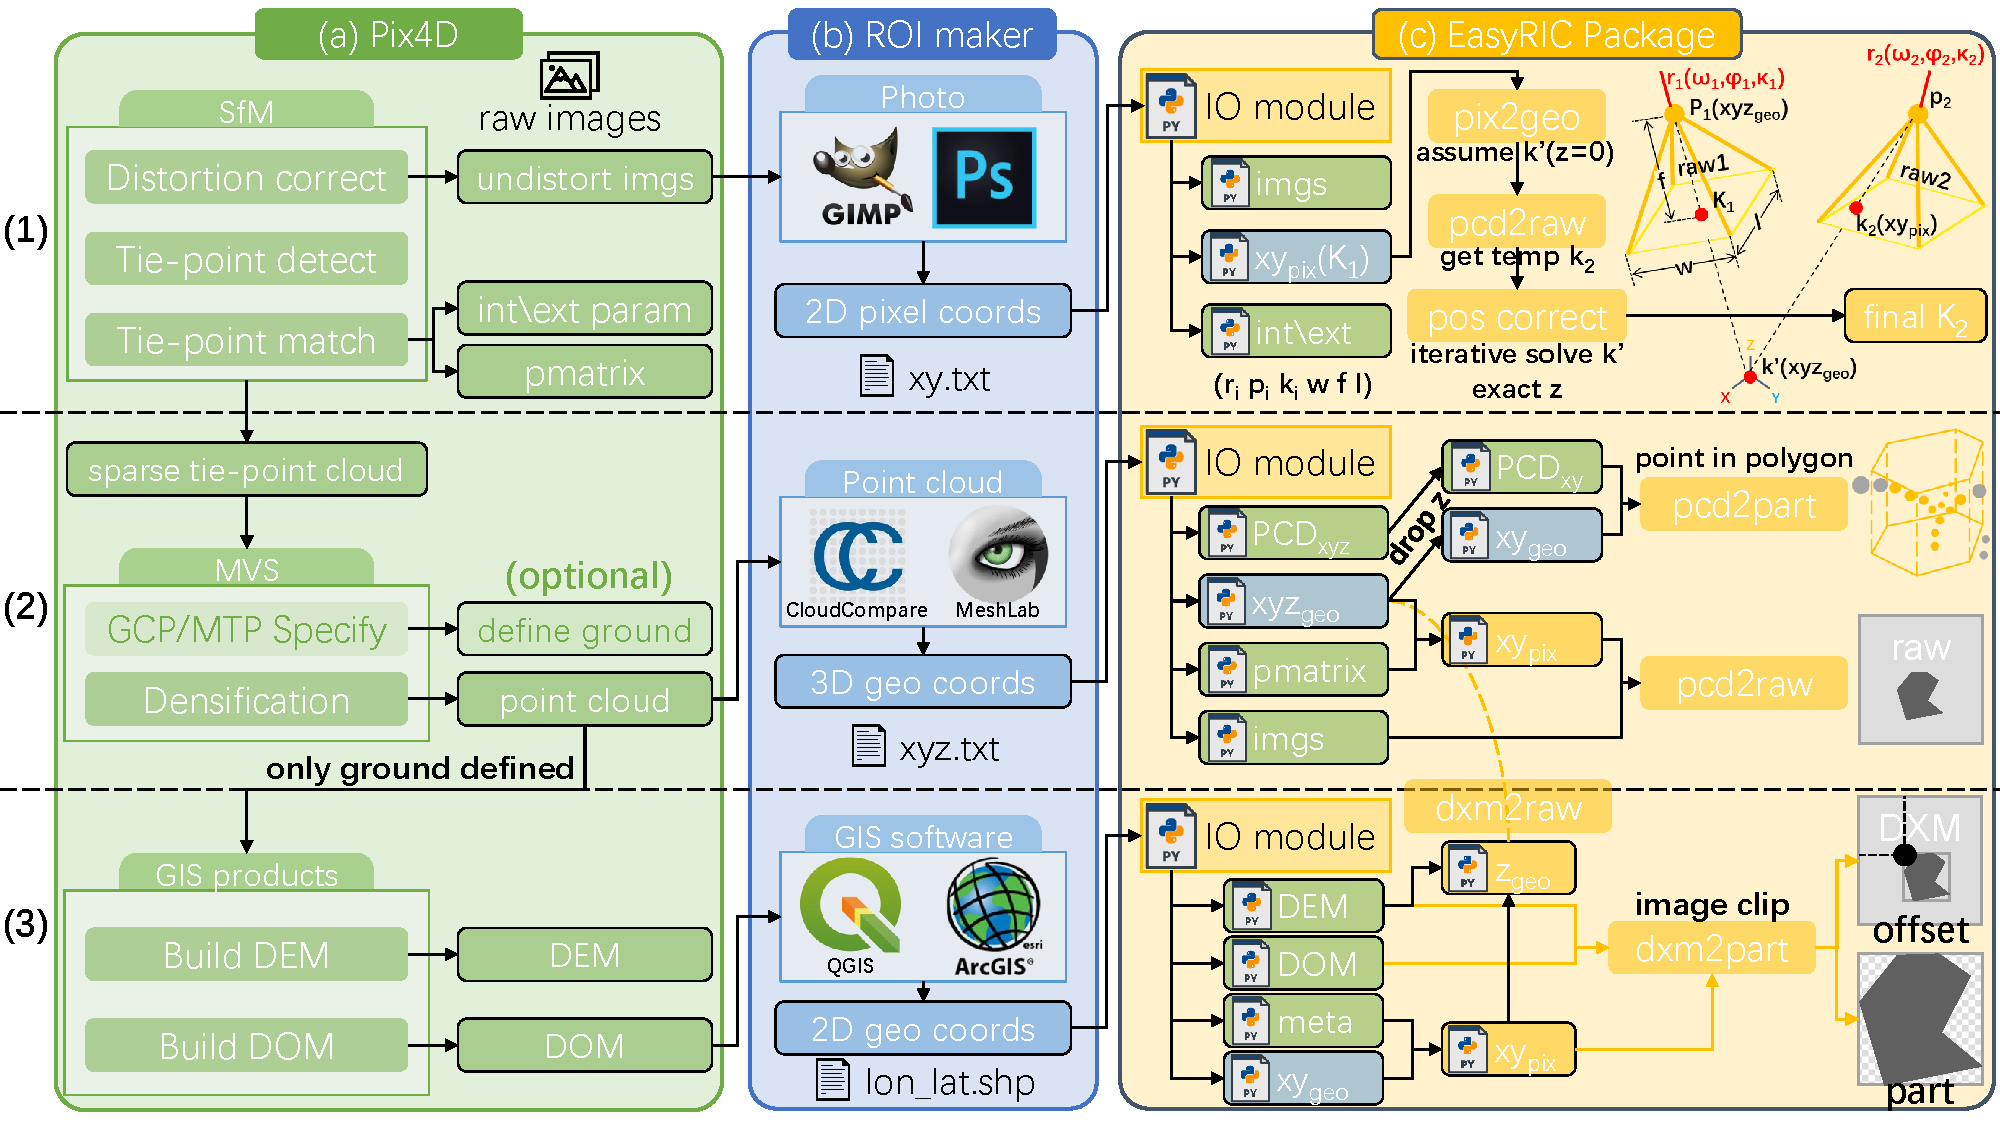
\includegraphics[width=0.95\linewidth]{figures/workflow.pdf}
  \caption{The workflow of proposed method. After obtaining image data, the 3D reconstruction (SfM-MVS) software is used to generate outputs of each processing step. Then the \acrfull*{roi} is marked via external commercial or open source tools. Finally, the EasyRIC package is used to deal with and connect between different SfM-MVS outputs and ROI, including reverse calculating the projected position of ROI and clipping the output by ROI ranges.}
  \label{fig:workflow}
\end{figure}

\begin{figure}[!htb]
  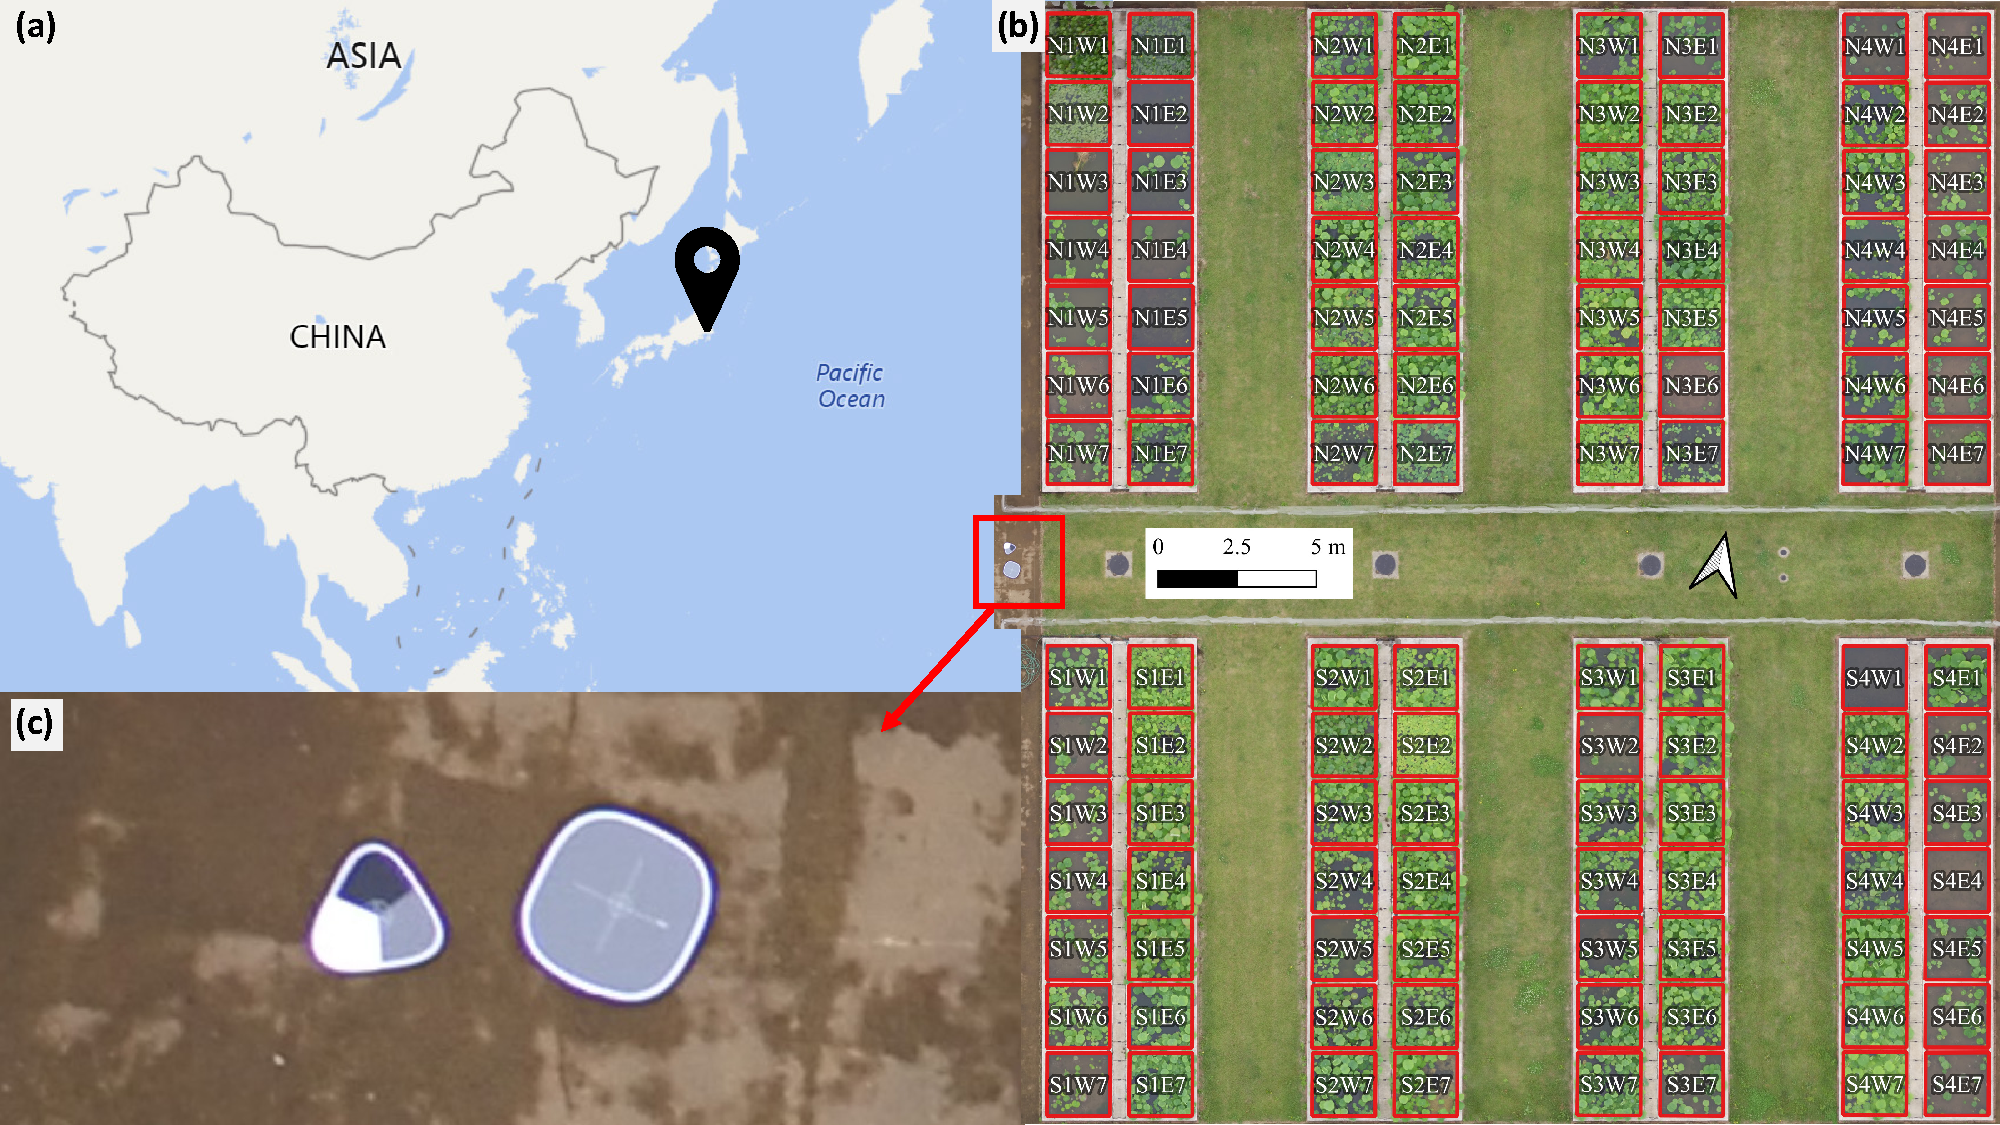
\includegraphics[width=0.95\linewidth]{figures/map.pdf}
  \caption{The experimental lotus plot condition. (\textbf{a}) the experimental plot locates in Nishi-Tokyo, Tokyo, Japan; (\textbf{b}) The labels of cultivation ponds, the orthomosaic showed here was collected on the May 5, 2017. The labels and boundaries of ponds were made by QGIS software and saved to shapefile (*.shp) for later usage; (\textbf{c}) shows the device used for obtaining geographic position and functioning as ground control point to linking different flight time series together}
  \label{fig:map}
\end{figure}

\begin{figure}[!htb]
  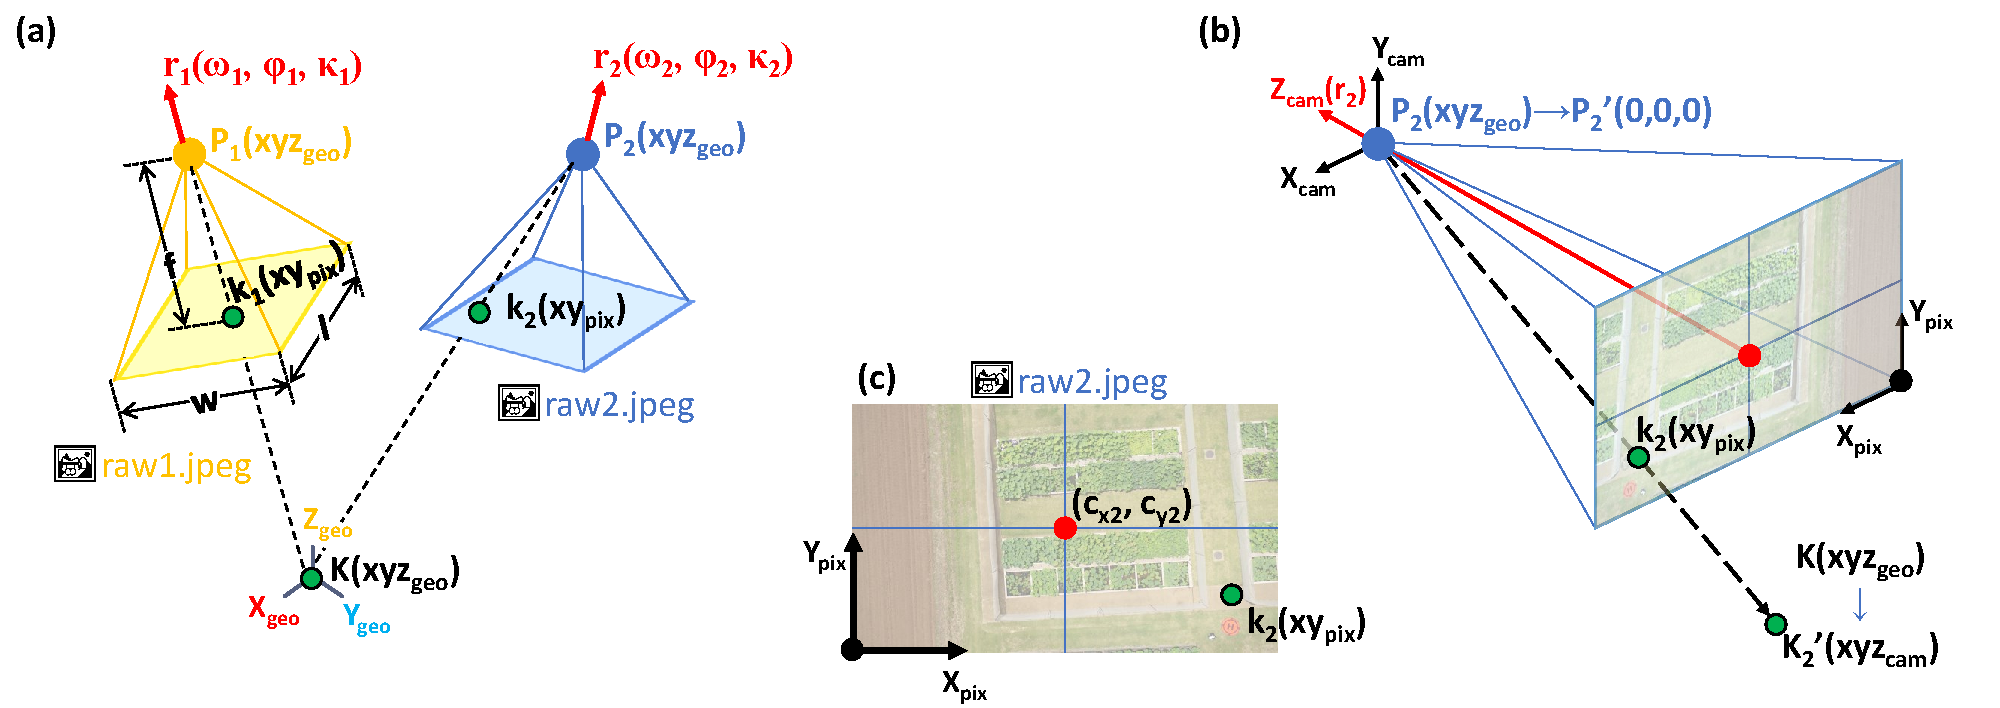
\includegraphics[width=0.95\linewidth]{figures/raw2raw.pdf}
  \caption{The geometry of camera model and 3D reconstruction. There are three different coordinate systems involved: real world coordinate system ($xyz_{geo}$, \textbf{a}), camera coordinate system ($xyz_{cam}$, \textbf{b}), and image coordinate system ($xy_{pix}$, \textbf{c} in pixel). (\textbf{a}) shows how a point in real world being recorded in different raw images, and $r_i$ represents camera rotation of raw image $i$; $P_i$, represents camera position of image $i$; $k_i$ represents 2D pixel coordinates on image $i$; $w$ is sensor width (mm); $f$ is sensor focal length, and $l$ is sensor length (mm). (\textbf{b}) offsets camera position to (0,0,0) for better linking pixel coordinate position ($k_i$) with real world position, where ($c_{x_i}$, $c_{y_i}$) is the image pixel center.}
  \label{fig:geom}
\end{figure}

\begin{figure}[!htb]
  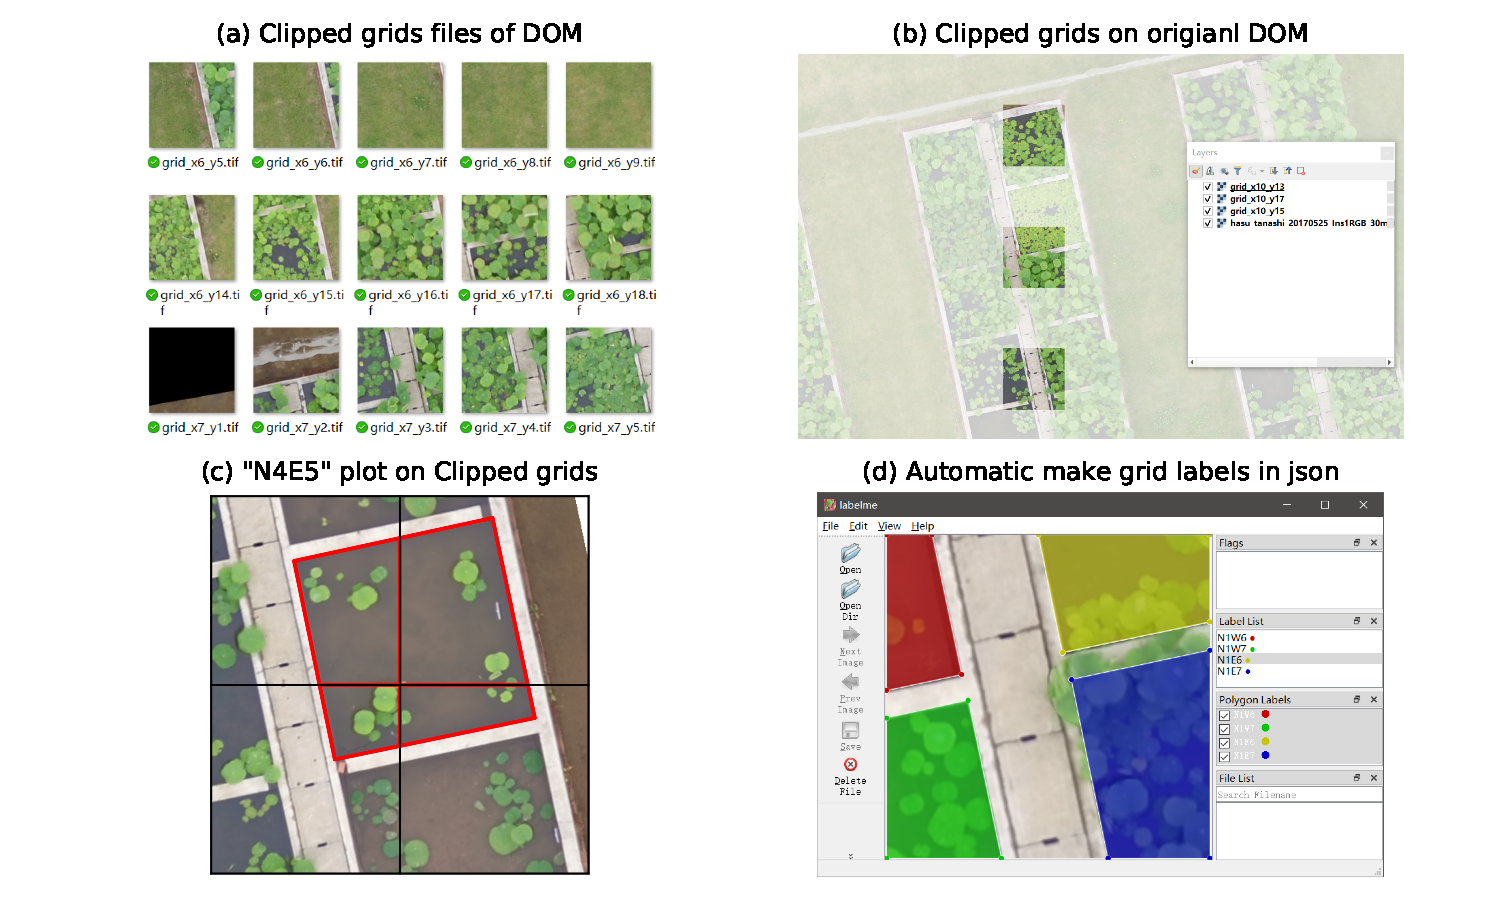
\includegraphics[width=0.95\linewidth]{figures/dom2grids.pdf}
  \caption{The example for \acrfull*{dom} grid clipping by given size. (\textbf{a}) showed the output geotiff files of clipped girds in windows 10 file management system. (\textbf{b}) showed the saved geotiff files contains the geographic information which can be overlaid the same position over original DOM in QGIS interface. (\textbf{c}) showed the clipping of given ROI according to each grid. (\textbf{d}) for each grid, different ROI sectors could be summarized and save to annotation json file (readable into LabelMe annotation software)}
  \label{fig:dom2girds}
\end{figure}

\begin{figure}[!htb]
  \includegraphics[width=0.95\linewidth]{figures/roi2dxm.pdf}
  \caption{The example for \acrfull*{roi} transformation between different \acrfull*{dom}, \acrfull*{pcd} and raw images. (\textbf{a}) showed the ROI marked by QGIS and displayed on DOM. (\textbf{b}) showed the clipped sector of DOM by ROI. (\textbf{c}) showed the ROI on PCD and (\textbf{d}) is the clipped PCD by ROI. (\textbf{e}) showed the ROI transformation results on raw images.}
  \label{fig:roi2dxm}
\end{figure}

\begin{figure}[!htb]
  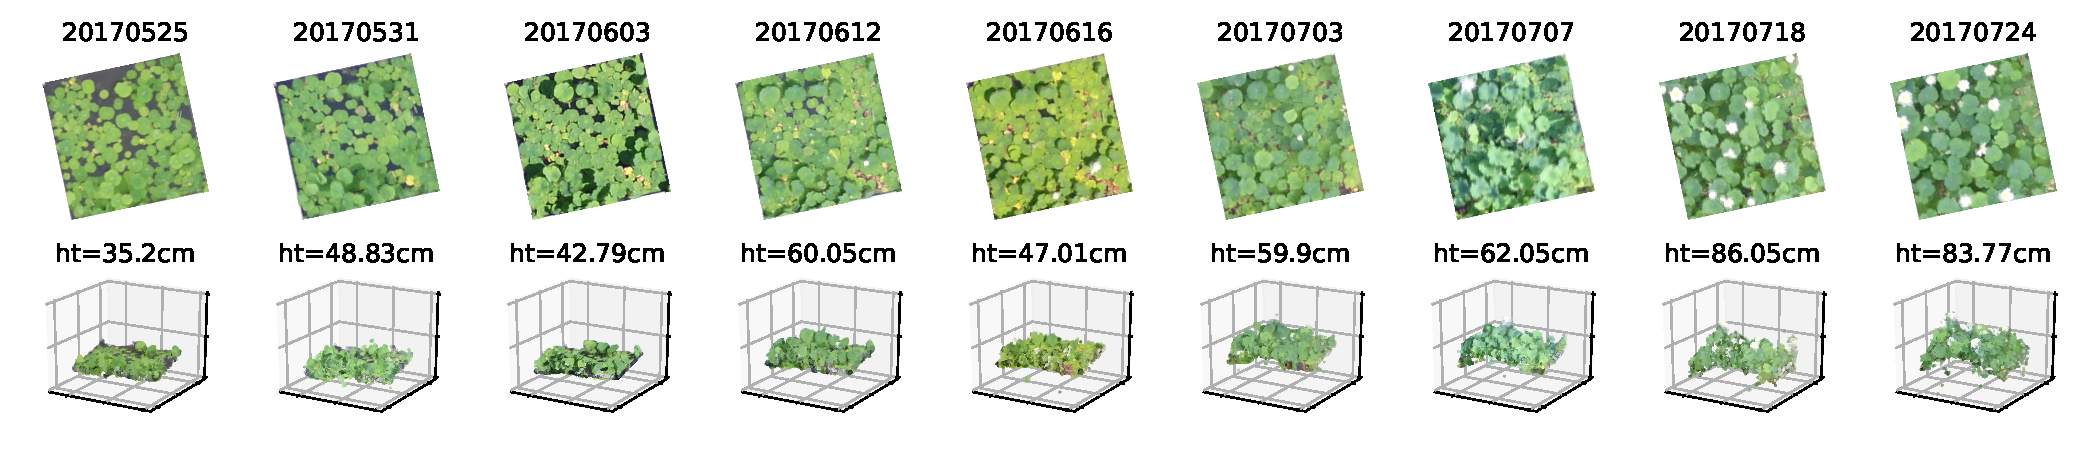
\includegraphics[width=0.95\linewidth]{figures/time_series.pdf}
  \caption{The time-series tracking of ROI, S2E1 plot as example, ranging from May 25 to July 24, 2017.}
  \label{fig:time}
\end{figure}

\begin{figure}[!htb]
  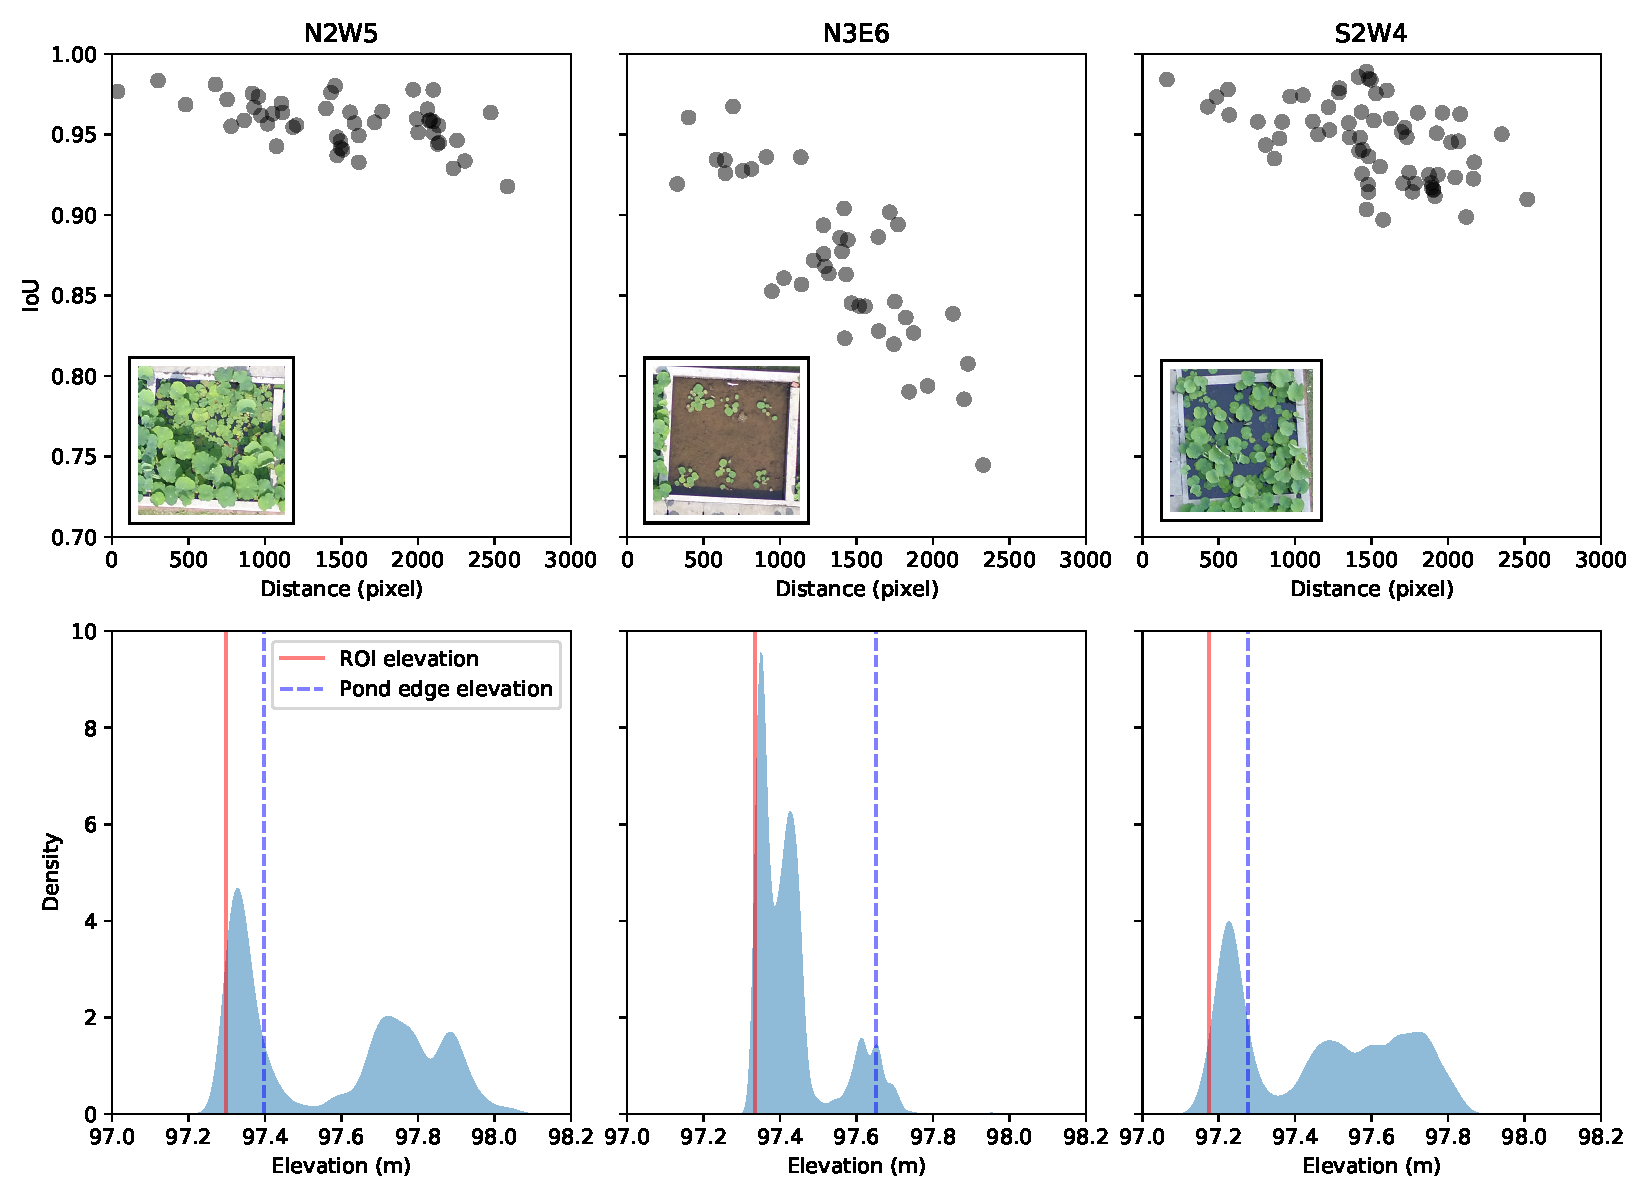
\includegraphics[width=0.95\linewidth]{figures/dist.pdf}
  \caption{The transformation accuracy examine results by fully manual marked plots. Three plots with different lotus leaf density and height were selected. All the expected ROI transformation positions were marked manually on related raw images by LabelMe annotation software. The distance is the Euclidean pixel distance from \acrfull*{iou} center to photo center. The distribution of each pixel point height is shown in blue area, the height of ROI (red solid lines) was the mean value of all pixel points smaller than 5 percentile threshold, and the height of pond edge (blue broken lines) was the mean value of random 10 points picked in QGIS on DSM.}
  \label{fig:dist}
\end{figure}

\begin{figure}[!htb]
  \includegraphics[width=0.95\linewidth]{figures/diff_ht.pdf}
  \caption{The effects of ROI position and ROI height for transformation. (\textbf{a}) shows three different height choices of ROI (5\% percentile, mean, 95\% percentile) by point cloud display. (\textbf{b}) and (\textbf{c})shows two different ROI position on raw images and related ROI transformation results.}
  \label{fig:ht_diff}
\end{figure}

\begin{figure}[!htb]
  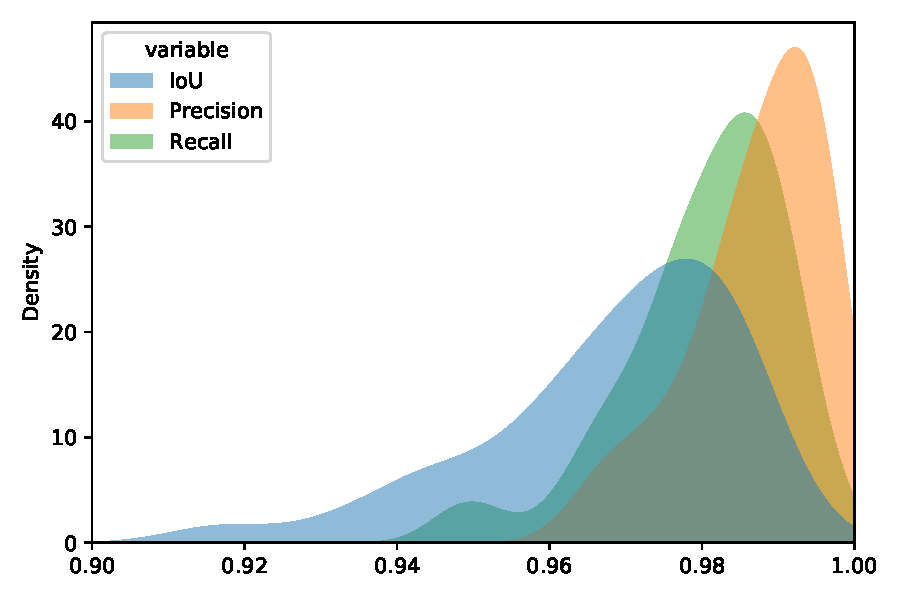
\includegraphics[width=0.95\linewidth]{figures/iou_all.pdf}
  \caption{The distribution of transformation accuracy indicators for central manual marked of all 112 lotus plots. For each plot, only those raw images with the smallest Euclidean pixel distance from ROI to image center were selected and manually marked.}
  \label{fig:iou_all}
\end{figure}

\begin{figure}[!htb]
  \includegraphics[width=0.95\linewidth]{figures/dl.pdf}
  \caption{Potential use for deep learning training data augmentation. Firstly, the DOM was clipped to 500px$\times$500px grids, the grid "x6-y7" was marked 6 annotation rectangles for lotus flowers by LabelMe. The annotation json file was imported to EasyRIC and did reverse calculation to all raw images. The "div" means the distance from annotation center to image center, smaller means closer to image center}
  \label{fig:dl}
\end{figure}

\end{backmatter}

\end{document}